
\documentclass[12pt]{article}
\usepackage{times}
\usepackage{setspace}
\setstretch{1.5}
\usepackage{amsmath,amssymb, amsthm}
\usepackage{graphicx}
\usepackage{bm}
\usepackage[hang, flushmargin]{footmisc}
\usepackage[colorlinks=true]{hyperref}
\usepackage[nameinlink]{cleveref}
\usepackage{footnotebackref}
\usepackage{url}
\usepackage{listings}
\usepackage[most]{tcolorbox}
\usepackage{inconsolata}
\usepackage[papersize={8.5in,11in}, margin=1in]{geometry}
\usepackage{float}
\usepackage{caption}
\usepackage{esint}
\usepackage{url}
\usepackage{enumitem}
\usepackage{subfig}
\usepackage{wasysym}
\newcommand{\ilcode}{\texttt}
\newcommand{\p}{\partial}
\usepackage{etoolbox}
\usepackage{physics}
\usepackage{xcolor}
\patchcmd{\thebibliography}{\section*{\refname}}{}{}{}



\makeatletter
\renewcommand{\@seccntformat}[1]{}
\makeatother

\begin{document}



\title{\textbf{CSDS 440: Assignment 5}}

\author{Shaochen (Henry) ZHONG, \ilcode{sxz517} \\ Mingyang TIE, \ilcode{mxt497}}
\date{Due on 10/09/2020, submitted \textcolor{blue}{early} on 10/02/2020 \\ Fall 2020, Dr. Ray}
\maketitle


% % % % % % % % % % % % % % % % % % % % % % % % % % % % % % % % % %
% % % % % % % % % % % % % % % % % % % % % % % % % % % % % % % % % %
% % % % % % % % % % % % % % % % % % % % % % % % % % % % % % % % % %
\section{Problem 19}

\begin{align*}
    b^T u &= u^T b \\
    &\leq u^T \cdot Ax \ \ \text{(Since $Ax \geq b$)}\\
    c^T X &= x^T c \\
    &\geq x^T A^T u \ \ \text{(Since $A^T u \leq c$)}\\
    &\geq u^T Ax \\
    \Rightarrow \ b^T u &\leq u^T Ax \leq c^T X \\
    \Longrightarrow \ b^T u &\leq c^T X
\end{align*}

The statement is therefore proven.

% % % % % % % % % % % % % % % % % % % % % % % % % % % % % % % % % %
% % % % % % % % % % % % % % % % % % % % % % % % % % % % % % % % % %
% % % % % % % % % % % % % % % % % % % % % % % % % % % % % % % % % %
\section{Problem 20}


We denote $h(u)$ to be the activation function for $u$ and we do not make assumption of which activation function is used (so we won't have the sigmoid simplication of $\frac{\partial h}{\partial u} = h(u)(1-h(u))$). For traning example $\alpha$, $h(\alpha) = o_\alpha$ (representing the prediction output), and we denotes $y = y_\alpha$ for the output label.

For the ease of understanding, we denote our symbols with respect to the following NN, which use almost identical notation to the one taught in \textit{Lecture 10}.\newline

\begin{figure}[H]
    \centering
    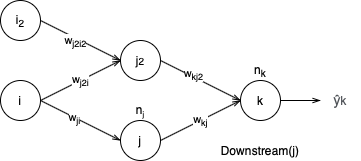
\includegraphics[width=0.6\linewidth]{{fig/fig_p20.png}}
\end{figure}


\subsection{Hidden-to-Output}

\begin{align*}
    \frac{\p L}{\p w_{ji}} &= \frac{\p L}{\p n_j} \frac{\p n_j}{w_{ji}} \\
    &= \frac{\p L}{\p n_j} \cdot \frac{\p (w_{ji} \cdot x_{ji})}{w_{ji}} \\
    &= \frac{\p L}{\p n_j} \cdot x_{ji} \\
    &= \frac{\p L}{\p h(n_j)} \frac{\p h(n_j)}{\p n_j} \ \cdot x_{ji} \\
    &= \frac{\p}{\p h(n_j)}(-y \log(h(n_j)) - (1-y) \log(1 - h(n_j))) \ \cdot \frac{\p h(n_j)}{\p n_j} \ \cdot x_{ji} \\
    &= (-\frac{-y}{h(n_j)} + \frac{1-y}{1- h(n_j)}) \ \cdot \frac{\p h(n_j)}{\p n_j} \ \cdot x_{ji} \\
    &= (\frac{1-y}{1- h(n_j)} -\frac{-y}{h(n_j)})\ \cdot \frac{\p h(n_j)}{\p n_j} \ \cdot x_{ji} \\
\end{align*}

Base on the calucation of the output layer, we may tall the backpropagation weight updates for hidden-to-output layer is:

\begin{equation*}
    \frac{\p L}{\p w_{ji}} = (\frac{1-y}{1- h(n_j)} -\frac{-y}{h(n_j)})\ \cdot \frac{\p h(n_j)}{\p n_j} \ \cdot x_{ji}
\end{equation*}

\subsection{Input-to-Hidden}

Since $j$ affects the $\hat{y}$ outputs only through $Downstream(j)$, we have:


\begin{align*}
    \frac{\p L}{\p w_{ji}} &= \frac{\p L}{\p n_j} \cdot \frac{\p n_j}{\p w_{ji}} \\
    &= \frac{\p L}{\p n_j} \cdot \frac{\p (w_{ji} \cdot x_{ji})}{w_{ji}} \\
    &= \frac{\p L}{\p n_j} \ \cdot x_{ji} \\
    &= \sum_{k \in Downstream(j)} \frac{\p L}{\p n_k} \cdot \frac{\p n_k}{\p n_j} \ \cdot x_{ji} \\
    &= \sum_{k \in Downstream(j)} \frac{\p L}{\p n_k} \cdot \frac{\p (w_{kj}h(n_j)}{\p n_j} \ \cdot x_{ji} \\
    &= \sum_{k \in Downstream(j)} \frac{\p L}{\p n_k} \cdot w_{kj}\frac{\p h(n_j)}{\p n_j} \ \cdot x_{ji} \\
    &= \frac{\p h(n_j)}{\p n_j} \cdot \sum_{k \in Downstream(j)} \frac{\p L}{\p n_k} \cdot w_{kj} \ \cdot x_{ji} \\
    &= \frac{\p h(n_j)}{\p n_j} x_{ji}  \cdot \sum_{k \in Downstream(j)} \frac{\p L}{\p w_{kj}} \frac{w_{kj}}{x_{kj}}
\end{align*}


Base on the calucation of the hidden layer, we may tall the backpropagation weight updates for input-to-output layer is:

\begin{equation*}
    \frac{\p L}{\p w_{ji}} = \frac{\p h(n_j)}{\p n_j} x_{ji}  \cdot \sum_{k \in Downstream(j)} \frac{\p L}{\p w_{kj}} \frac{w_{kj}}{x_{kj}}
\end{equation*}

% % % % % % % % % % % % % % % % % % % % % % % % % % % % % % % % % %
% % % % % % % % % % % % % % % % % % % % % % % % % % % % % % % % % %
% % % % % % % % % % % % % % % % % % % % % % % % % % % % % % % % % %
\section{Problem 21}

Note for the following neural network, the weights are noted on the edges and the activation thresholds are noted on the top of each neuron (as for the neuron with threshold $x$ will output $+1$ if the input $\geq x$, and output $-1$ otherwise). Note we omitted $x_2$ as it is simply a duplication of $x_1$, and we can design a network without using the former.

\begin{figure}[H]
    \centering
    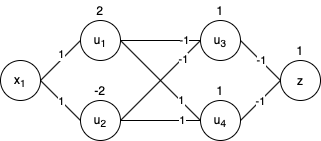
\includegraphics[width=0.6\linewidth]{{fig/fig_p21.png}}
\end{figure}

Now to trace each example. Note for each neuron, the inequality is the input against the activation threshold and the output is the one in bracket.
\begin{table}[H]
\centering
    \begin{tabular}{|rr|rrrr|r|}
        \hline
        $x_1$ & $x_2$ & $u_1$ & $u_2$ & $u_3$ & $u_4$ & $z$ \\
        \hline
        -4 & -4 & $-4<2$ (-1) & $-4< -2$ \ (-1) & $1 + 1 > 1$ \ (1) & $-1 - 1 < 1$ \ (-1) & $-1 + 1 < 1$ \ (-1) \\
        -1 & -1 & $-1<2$ \ (-1) &$-1> -2$ \ (1)  & $1 - 1 < 1$ \ (-1) & $1 - 1 < 1$ \ (-1) & $1 + 1 > 1$ \ (1) \\
        1 & 1 &  $1<2$ \ (-1) &  $1>-2$ \ (1)& $1 - 1 < 1$ \ (-1) & $1 - 1 < 1$ \ (-1) & $1 + 1 > 1$ \ (1) \\
        4 & 4 & $4>2$ (1) & $4>-2$ \ (1) & $1 - 1 < 1$ \ (-1) & $1 + 1 > 1$ \ (1) & $1 - 1 < 1$ \ (-1) \\
        \hline
    \end{tabular}
\end{table}

We have showed the network is able to produce the correct classification.


% % % % % % % % % % % % % % % % % % % % % % % % % % % % % % % % % %
% % % % % % % % % % % % % % % % % % % % % % % % % % % % % % % % % %
% % % % % % % % % % % % % % % % % % % % % % % % % % % % % % % % % %
\section{Problem 22}

I asked TA, couple of my classmates, and consulted online resources. It seems there are two ways to answer this question. One is to calculate the gradient between each layer and show that without the $sign()$ function the weight will stop updating, but it does not utilized the hint of decision boundary.\newline

So a conceptual argument can be formed on the idea of if we drop the $sign()$ function, a neuron's activation function will simply be its input -- which is a linear function of all pervious neurons. This suggests the output of the ANN will also be a linear function of the input, as combination of linear function is always linear. Thus the ANN will have a linear decision boundary, which voids the purpose of having a deep network (as we can rewrite the whole network with just a single layer), and such network won't be useful for solving a problem which requires a non-linear decision boundary.\newline

\noindent Below is the gradient calculation approach.




\begin{figure}[H]
    \centering
    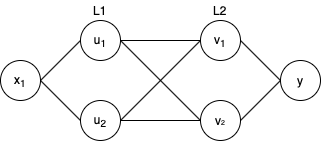
\includegraphics[width=0.4\linewidth]{{fig/fig_p22.png}}
\end{figure}


Assume we have the above ANN of two hidden layers, each with $m$ number of nerons, a common square loss will be:


\begin{align*}
    L(w) &= \frac{1}{2} \sum_{i = 1}^m (y_i - \hat{y_i})^2 \\
    &= \frac{1}{2} \sum_{i = 1}^m (y_i - sign(w \cdot x_i))^2
\end{align*}

For the sake having something differentiable, we drop the $sign()$ function and make it as:

\begin{equation*}
    L(w) = \frac{1}{2} \sum_{i = 1}^m (y_i - w \cdot x_i)^2
\end{equation*}

Therefore, for the gradient of $L_2$ and output, we have:

\begin{align*}
    \frac{\p L_2}{\p w} &= \sum_{i}^{m} (y_i - w \cdot x_i)(-x_i) \\
    &=\sum_{i}^{m} (w \cdot x_i^2 - x_i \cdot y_i)
\end{align*}

We furter differentiate it to get the gradient of $L_1$ and $L_2$:

\begin{align*}
    \frac{\p L_1}{\p w} &= \frac{\p}{\p w} (\sum_{i}^{m} (w \cdot x_i^2 - x_i \cdot y_i)) \\
    &= \sum_{i}^{m} x_i^2
\end{align*}

Similiarily, for gradient of input and $L_1$

\begin{equation*}
    \frac{\p L_{\text{input}}}{\p w} &= \frac{\p}{\p w} \sum_{i}^{m} x_i^2 = 0
\end{equation*}

Since the gradient is 0, the weight of the input will not be updated. Note this is just a 2-layer ANN, an arbitrary ANN with more layers but without the $sign()$ function might also encounter this problem and make the weight updating mechanism ineffective.


% % % % % % % % % % % % % % % % % % % % % % % % % % % % % % % % % %
% % % % % % % % % % % % % % % % % % % % % % % % % % % % % % % % % %
% % % % % % % % % % % % % % % % % % % % % % % % % % % % % % % % % %
% \section{References}
% \nocite{*}
% \raggedright
% \bibliography{references.bib}
% \bibliographystyle{plain}


\end{document}